\scanpage{95}
Il faudrait aussi, de façon générale (dans le contexte ``quasi'') étudier
\deleted{\unsure{le}} si $H^i(k,G)$ peut se calculer comme une cohomologie
galoisienne\ldots
\margin{\figure{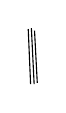
\begin{tikzpicture}[x=1cm,y=1cm]
\draw (0,0)--(-.03,.7); \draw (.045,0)--(.01,.71); \draw (.085,.015)--(.05,.68);
\end{tikzpicture}}}

\deleted{N.B. Il n'y \unsure{a pas} \illegible{3} \unsure{élémentaire} de
Weil \unsure{permette}.}
\mspage{94}

